\newcommand{\RecoTrack}{\texttt{RecoTrack}\ }
\newcommand{\Track}{\texttt{genfit::Track}\ }
\newcommand{\Hit}{\texttt{RecoHitInformation}\ }
\chapter{Additional software changes} \label{chapter-addon}

This chapter summarizes some of the additional changes made to basf2 during the writing of this thesis for documentation purposes. They all stay in relation to the changes made for the tracking framework but do not try to increase the physical figures of merit or alike. They are listed here without a special ordering or connections.

\section{\texttt{RecoTrack}}
As described in chapter~\ref{chapter-vxd}, the former \Track and the \texttt{genfit::TrackCand} were merged together to form a new \RecoTrack class which is described with its accompanying models in the following. The motivation was to create a better interface to the fitting algorithms provided by the genfit package and to fit seamlessly into the data store structure. As one of the goals of the genfit package is to stay as general as possible, this structure can not be incorporate tightly into the fitting algorithms. Instead, a wrapper class is built which inherits both from the \Track and from the \texttt{RelationInterface} in form of a public inheritance 
\begin{center}
  \lstset{escapechar=@,style=customC}
  \lstinline@ class RecoTrack : public RelationInterface<genfit::Track> { ... }@
\end{center}
which turns the \RecoTrack into a drop-in-replacement for the \Track as all algorithms of genfit work with \Track objects. 

In the first subsection, the \RecoTrack dataobject is described in more detail whereas the second subsection describes the needed environmental modules.

\subsection{\RecoTrack and \Hit}

The \Track objects are containers for a list of \texttt{genfit::TrackPoint} pointers with one or few \texttt{AbstractMeasurement} in each of them (see chapter~\ref{chapter-vxd} for more information on the measurements). These track points are needed for the fitting algorithm and include not only the hit information but also sorting parameters and additional information like the detector where this hit was found. On the other side are the raw hit information coming from the detector that get written to several StoreArrays. These raw hit classes, namely \texttt{CDCHit}, \texttt{SVDHit} and \texttt{PXDHit} are used by the track finding algorithms and have to be transformed into the track points needed by genfit. To encapsulate the track finding from the track fitting, this step is not included in the finder modules, also because the track points can not be saved into StoreArrays and written into ROOT output files. The \RecoTrack needs to handle both hit types: the track points and the raw hits. Therefore, the raw hits are saved as relations to the \RecoTrack instances (this is possible as the raw hits as well as the \RecoTrack inherit from \texttt{RelationInterface}) and then turned into track points by the \texttt{MeasurementCreatorModule} (again see chapter~\ref{chapter-vxd} for more details). These points are stored in the parent \Track itself as a \texttt{std::vector}. This approach together with some methods of the \RecoTrack to access and receive hit information conveniently makes the \RecoTrack relatively lightweight as it does not have to store lists of raw hits in addition.

One problem with this approach is, that it is impossible to store additional information like the sorting order of the hits or the track finder which has found the hit, as the relation can only be used to store one additional \texttt{double} value together with each pair. To solve this issue, a second dataobject -- the \Hit -- was created to store these additional information. When adding a raw hit to the \RecoTrack a \Hit instance is created automatically and stored with relations to the raw hit and the \RecoTrack, which leads to the triangular shaped relation diagram shown in figure~\ref{fig-reco-hit-relation}. As the \RecoTrack has already buildin functions to access the additional information in a convenient way, there is no need for the user of the dataobject to take care of the \Hit instances by himself. 

\begin{figure}
  \centering
  \begin{tikzpicture}[thick]
    \node[module, text width=10em, fill=kit-orange50] (track) {\RecoTrack};
    \node[module, text width=10em, fill=kit-orange50, right=6.0 of track] (hit) {\Hit};
    \node[module, text width=10em, fill=kit-orange50, below right=of track] (cdchit) {\texttt{CDCHit}};

    \draw[vecArrow, <->] (track) -- (hit) node [midway, above] {1:n};
    \draw[vecArrow, <->] (cdchit) -- (hit) node [midway, below] {1:p};
    \draw[vecArrow, <->] (track) -- (cdchit) node [midway, below] {m:k};
  \end{tikzpicture}
  \caption[Relation diagram between \RecoTrack, \Hit and raw hits.]{Relation diagram between the two newly created dataobjects \RecoTrack and \Hit and one raw hit. The arrows describe the relation between the objects which are accessible in both ways. The numbers on the arrows describe the cardinality of the relation. These cardinalities are the reason why the relation diagram can not be reduced further.}
  \label{fig-reco-hit-relation}
\end{figure}

Together with the already described convenience-functions to add and receive raw hit information the \RecoTrack also includes a method to prepare the underlaying \Track for the fitting algorithm. This includes setting the time seed information and adding a representation instance which stores the particle type information.

\subsection{Modules for the \RecoTrack}

Together with the \RecoTrack dataobject, four modules where written which altogether have the same functionalities as the \texttt{GenfitterModule} but split up to improve the configurability. These modules are
\begin{description}
 \item[RecoTrackCreatorModule] Although the \RecoTrack should replace the \texttt{genfit::Track\-Cand} in the future, it is easily possible to include the \RecoTrack workflow into the module path without rewriting all the track finder modules with the \texttt{Reco\-Track\-Creator\-Module}. The module transforms an ingoing StoreArray of \texttt{genfit::\ Track\-Cand} objects into \RecoTrack instances and creates the needed relations between the track candidates and the tracks.
 \item[MeasurementCreatorModule] This module is responsible for transforming the added raw hits of the \RecoTrack into track points. It uses highly configurable \texttt{MeasurementCreatorFactory} objects which can add arbitrary track points (which is used for adding the momentum estimations in the VXD) out of the raw hits added by the track finding algorithms. A sketch of the working principle of the module can be found in figure~\ref{fig-measurement-creator}.
 \item[BaseFitterModule] This module and its derived modules \texttt{KalmanRecoFitter} and \texttt{DAF\-Reco\-Fitter} are responsible for creating an object of the genfit fitting algorithm and passing this to every \RecoTrack to use it for fitting. When doing this, also the preparation functions for the fit are called.
 \item[TrackBuilderFromRecoTracksModule] In the end, not the whole track but only the perigee parameters are important for the physics analysis. Therefore this module extrapolates the tracks to the perigee with the extrapolation methods provided by genfit. It saves its results in \texttt{Belle2::Track} objects which are used in the analysis later.
\end{description}

The named modules together with the \texttt{SetupGenfitExtrapolationModule} in front of them should run in the given order in the usual use case.

\begin{figure}
  \centering
  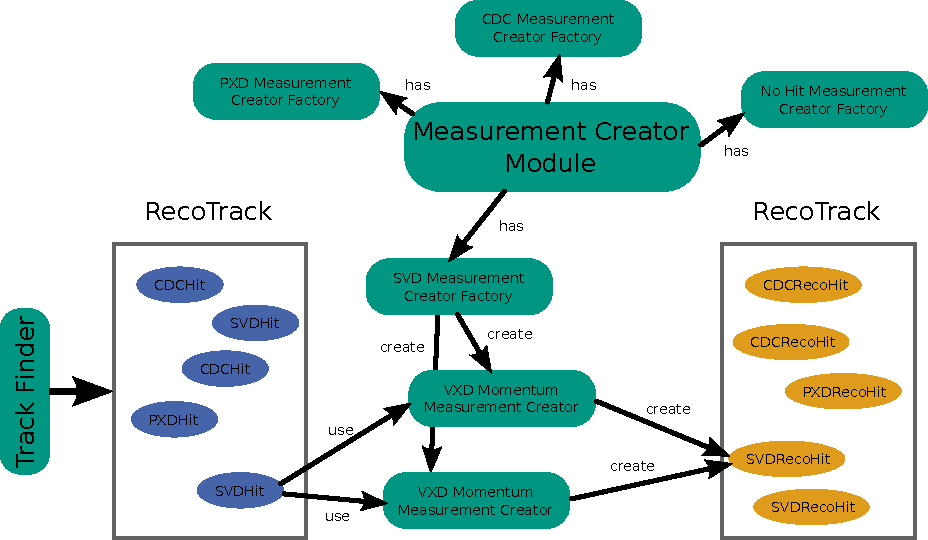
\includegraphics[width=\linewidth]{figures/vxd/measurementCreator.pdf}
  \caption[Diagram showing the creation of measurements.]{Diagram showing the creation of measurements in the \texttt{MeasurementCreatorModule} as described in the text. Each \texttt{RecoTrack} includes PXD, SVD and CDC hits (blue) added by the track finder algorithms which must be transformed into \texttt{AbsMeasurement} objects (orange) to be handled by the track fitting routine later. These measurements can include positional, directional and/or $q/p$ coordinate values with their errors.}
  \label{fig-measurement-creator}
\end{figure}


\section{IPython interface for basf2}

IPython (or jupyter as it is now called~\cite{jupyter}) is an application which provides interactive computing including an interactive shell and a client-server structure for notebooks. It has support for many different languages (like C++, ROOT~\cite{root_ipython}, Haskell, Julia, R) and also for Python, which is included by default. Using IPython notebooks instead of raw python has many advantages, e.g.
\begin{itemize}
  \item context-sensitive tab completion which is better as the one provide by many IDEs, as it can use the duck-typing of the running python interpreter.
  \item syntax highlighting and automatic indention.
  \item inline graphics created with Python (e.g. matplotlib) and the possibility to include equations with \LaTeX, markdown comments, images and videos.
  \item well-organized notebook structure which can hold the script and the result in a structured way which makes it easily readable for other people.
  \item no additional programs needed as the notebook server is accessible with a standard HTML browser (making it possible to use smartphones, tablets and remote computers) or with plugins (for pycharm, emacs etc.)
\end{itemize}

All these mentioned points make IPython suitable for quick analysis in the tracking software development as well as for larger physics analysis which may be stored centralized and accessible for other developers to share thoughts and solutions. For calculating most of the results presented in this thesis, IPython notebooks were used. As the basf2 framework is not built for interactive use, a \texttt{ipython\_tools} python module was created which will be presented in the following.

The main entrance point of the module is a predefined handler object. For normal use cases, this is the only object one needs to import from the module. After importing the handler, the user can create the basf2 module path as in a normal steering file (see listing~\ref{lis-steering-file} for an example). Instead of using the normal basf2 process function, it is better to use the one provided by the handler. The calculation is sent as a different process to the background (using the \texttt{multiprocessing} module of python~\cite{multiprocessing}) and can be monitored using IPython instead of blocking the IPython notebook until it finishes. Also, in case of failure, the IPython notebook still keeps on running, making it possible to look into the log files of the process which get written to temporary files and can be accessed with the handler.

Calling \texttt{handler.process} with a path returns an instance of a \texttt{Basf2Calculation} which summarizes all properties and methods of a module path calculation. The calculation can be for instance started or stopped, the log or the running status can be accessed or the input parameters can be checked. Some example uses are shown in the notebook in listing~\ref{lis-calculation}. As can be seen in the listing, the notebook processing goes on although the path calculation is running. As it runs in a different process it is even possible to close the notebook running in the browser (but not the notebook kernel) and reaccess it e.g.\ from another device later with the path calculation still going on.

If the further results depend on the output of the path calculation or a status bar with the current percentage should be shown, the calculation offers a \verb+wait_for_end+-function which blocks until the background calculation is finished or has failed. For accessing the current percentage of the calculation, a small python module is included into the processed path on every call of \texttt{handler.process}. This module collects the current event number and the total number of events from the \texttt{Environment} singleton and sends it to a dedicated pipe attached to the background process running the path calculation and the foreground notebook. This value is constantly pulled and shown as a progress bar with timing estimation when the method \verb+wait_for_end+ is called until the calculation has terminated.

The \texttt{handler} associates to each path an instance of the \texttt{Basf2Queue} class. These queue objects mimic the behavior of a python dictionary as they can be filled with pairs of a string as a key and an arbitrary pickable python object as value with their \verb+get+ function. They can be used before, in or after the path processing as they get passed to the background process by a multiprocessing queue. They should store calculation-related information like the name of output and input files and are used extensively in the \texttt{ipython\_tools} to store for example the statistics of the calculation.

To increase the usability in the typical browser environment the IPython notebook is running, most of the output results of a path calculation are turned into mostly interactive HTML-widgets. Examples are the calculation statistics, the module path and the store array content which are accessible via the functions \verb+show_statistics+, \verb+show_path+ and \verb+show_collections+ of the \texttt{Basf2Calculation} objects.

One \texttt{Basf2Calculation} object can not only handle one single basf2 module path but also a list of them. The command to generate one calculation for many different paths is the method \verb+process_parameter_space+ of the \texttt{handler} object which is working like a grid search. This method expects a function \verb+path_creator+ returning basf2 paths and the same arguments as this function as keyword arguments. The values given to these arguments should be iterable objects as the \verb+process_parameter_space+ builds every argument combination and calls the \verb+path_creator+ with this.\footnote{One exception is, when using an argument called \texttt{queue} in the \texttt{path\_creator} function. No values for this argument can be provided as it gets automatically filled with queue objects by the \texttt{handler}.} The resulting lists of paths is then used to build a \texttt{Basf2Calculation} object. All the before mentioned methods and properties of the calculation work as expected also for lists of paths. Per default, they return a list of results -- one item for each path. Also, by supplying a non-negative number to the methods, the result of a certain path can be selected. The methods returning a widget return a tab viewer widget now, which includes all the resulting widgets for the different paths.

\begin{listing}
\begin{inputipynb}
from ipython_tools import handler
path = ...
calculation = handler.process(path)
\end{inputipynb}
\begin{inputipynb}
print calculation.get_status()
print calculation.is_running()
calculation.start()
print calculation.get_status()
print calculation.is_running()
\end{inputipynb}
\begin{outputipynb}
not started
False
running
True
\end{outputipynb}
\begin{inputipynb}
calculation.stop()
print calculation.get_log()
\end{inputipynb}
\begin{outputipynb}[\theipythcntr]
[INFO] Creating Geometry
[INFO] Creating geometry for detector: Belle2Detector
...
\end{outputipynb}

  \caption[Example use cases for the Basf2Calculation objects.]{Example use cases for the \texttt{Basf2Calculation} instance returned by a call to \texttt{handler.process}. As the process runs in the background, the IPython kernel can go on with the foreground calculation.}
  \label{lis-calculation}
\end{listing}

\section{Docker and the basf2 software}

Docker is an open-source-project~\cite{docker} which allows to package and ship arbitrary applications with all of its dependencies. It uses a standardized image format and runs its processes in specific cgroups and namespaces isolating the docker applications from the rest of the operation system. Running docker containers can share libraries and the kernel with the rest of the system decreasing the memory footprint of starting the same application more than once in parallel. The isolation and the smaller memory consumption compared to normal virtualization solutions (like VirtualBox) make the program suitable for batch systems or server applications.

A typical docker workflow consists of three steps:
\begin{description}
  \item[Create the docker image] Using a domain specific language the contents of a docker image can be defined. A docker image consists of different layers of the AuFS or btrfs filesystem which can contain a whole application with all its libraries and even the operation system. Because the images share resources with their host system, the size of such an image is typically in the order of only a few gigabytes.
  \item[Ship the docker image] The image can be extracted into a tar-ball keeping the layer structure which makes it possible to update the software more easily. Every docker user can extract the image and use it -- not depending on the kernel version or the operation system. To not mix up different images, docker has an inbuilt versioning system which can be used to give tags and labels to the images.
  \item[Run the docker image] Each time a docker image is started a new container is created with the form defined exactly by the image. Because of the underlaying filesystem only the changes performed in the running docker containers are stored. Starting the same image twice does therefore not imply to copy the libraries again. The docker processes are given a special cgroup with adjustable restrictions. Per default, the docker processes are not allowed to access the filesystem of the host machine or change kernel parameters which isolates the processes from the host. The docker container runs as long as the process in it is running and gets deleted after the process has finished.
\end{description}

The benefits of using docker like the easier distribution of software among heterogeneous systems typical for a collaboration, the small memory consumption even with multiple instances of the same application and the isolation can be used for various basf2-related tasks. Possible examples include
\begin{itemize}
 \item running the build bot as it is easy to test the compilation process against different operation systems or different library versions without the need to rebuild a physical computer,
 \item running the validation scripts and the unit tests as the containers run with a defined starting point making it impossible to create dependencies between consequent runs,
 \item doing a physics analysis as the setup time is rather low and the updating process is easy as the compilation can be performed by the image creator,
 \item providing server applications as the isolation of processes makes it even possible to give full access to remote users for example by exposing the access to a python interpreter.
\end{itemize}

Because of the numerous benefits, a docker image holding the full basf2 software components with all the needed dependencies was created in this thesis. It is built using the orchestration software ansible~\cite{ansible} to make the scripts reusable for other purposes like creating VirtualBox images or provisioning a server system. The ansible scripts download and compile the basf2 tools, externals and the software into a docker image which can then be started on a machine without the need for configuration or long-lasting compilations.

The docker software can be combined with the IPython concept presented before. Users can be given access to a docker container with a running IPython server instance. The users can then perform their calculations using the data and computing power provided by the host system without the need for installations on their local machine. Various concepts like the jupyterhub~\cite{jupyterhub} or the tmpnb-project~\cite{tmpnb} can be easily incorporated. 

\section{The \texttt{root\_pandas} module}

The ROOT data format is a high-efficient, strongly compressed storage format which is used extensively in high energy physics projects because of its benefits especially for typical experiment data of long tuples full of floating point numbers. Modern data analysis techniques however include the data processing with python and the python own modules like \texttt{pandas}~\cite{pandas} or \texttt{matplotlib}~\cite{matplotlib}. To close the gap between the in-memory database processor \texttt{pandas} and the ROOT data format the \texttt{root\_pandas} module was implemented in this thesis which is strongly based on the already available project with the same name~\cite{root-pandas}. The methods provided by the already developed module were rewritten to cope better with ROOT data files containing both numerical and non-numerical data and with large data files. The package provides mainly two functionalities. Both use the \texttt{root\_numpy}~\cite{root-numpy} package for the interconnection with ROOT.

\begin{description}
 \item[ROOT import] The \verb+read_root+ method can read ROOT files and export the \texttt{TNtuples} in the files to \texttt{pandas} data frames with each branch leading to one column of the same name. It can export single trees (by handing in a tree\_key argument) or for each tree in the file one data frame as a list. It automatically filters out non-numerical data. When giving the chunksize argument, the ROOT file gets split into chunks of the given size and a python generator object is returned which can be used to keep the data in memory small.
 \item[ROOT export] The \verb+to_root+ function can be used to export arbitrary pandas data frames to the ROOT format. The branch names are copied from the data frame.
\end{description}
